%%%%%%%%%%%%%%%%%%%%%%%%%%%%%
\section{Storms}
Written by Cédric Rolland \& Alexis Kessel.\\

Storms are usually characterised by violent winds and heavy rain. These extreme events can be local, like tornado, or more spread, like hurricanes. We detect these storms by looking for records containing high-speed winds and deduce some extreme events based on this information.

%%%%%%%%%%%%%%%%%%%%%%%%%%%%%
\subsection{Wind Threshold}
In order to identify a storm we had to find winds that overtake a certain threshold. The measures being in m/s * 10, we started by setting a value of 280 as used in the \href{http://en.wikipedia.org/wiki/Beaufort_scale}{Beaufort scale}. This scale sets the speed of wind of 103 km/h (28 m/s) as a boundary to consider the wind to be a violent storm or worse, a hurricane ($>$ 118 km/h).

An extreme event is not constant by nature and can last for days. The wind speed is also not constant and there is often some drop of speed during the event (while remaining pretty high). If we set the threshold at very high speed only we would not get the overall event but only some extreme part of it, and it would be detected as multiple extreme events. We finally found a threshold that allows us to have a lot of extreme events but in return we also have some less extreme events that are also shown, events with only weak wind and no extreme winds. Therefore we discard events where the max wind speed in under a certain threshold. This allows us to have complete extreme events with high and low wind speeds and not having events with low wind speed only.

We ended up setting the value of the min wind speed to 180 (~65km/h) and the second threshold to 280 (~100km/h) at the expense of the definition of the start date, and end date of the event, but which allowed us to better define the amplitude of the event.

The following figures show a storm and its corresponding Wikipedia article. This extreme event is the hurricane Andrew that hit Florida and New Orleans in 1992.
\begin{figure}[ht]
\centering
\makebox[\textwidth][c]{
  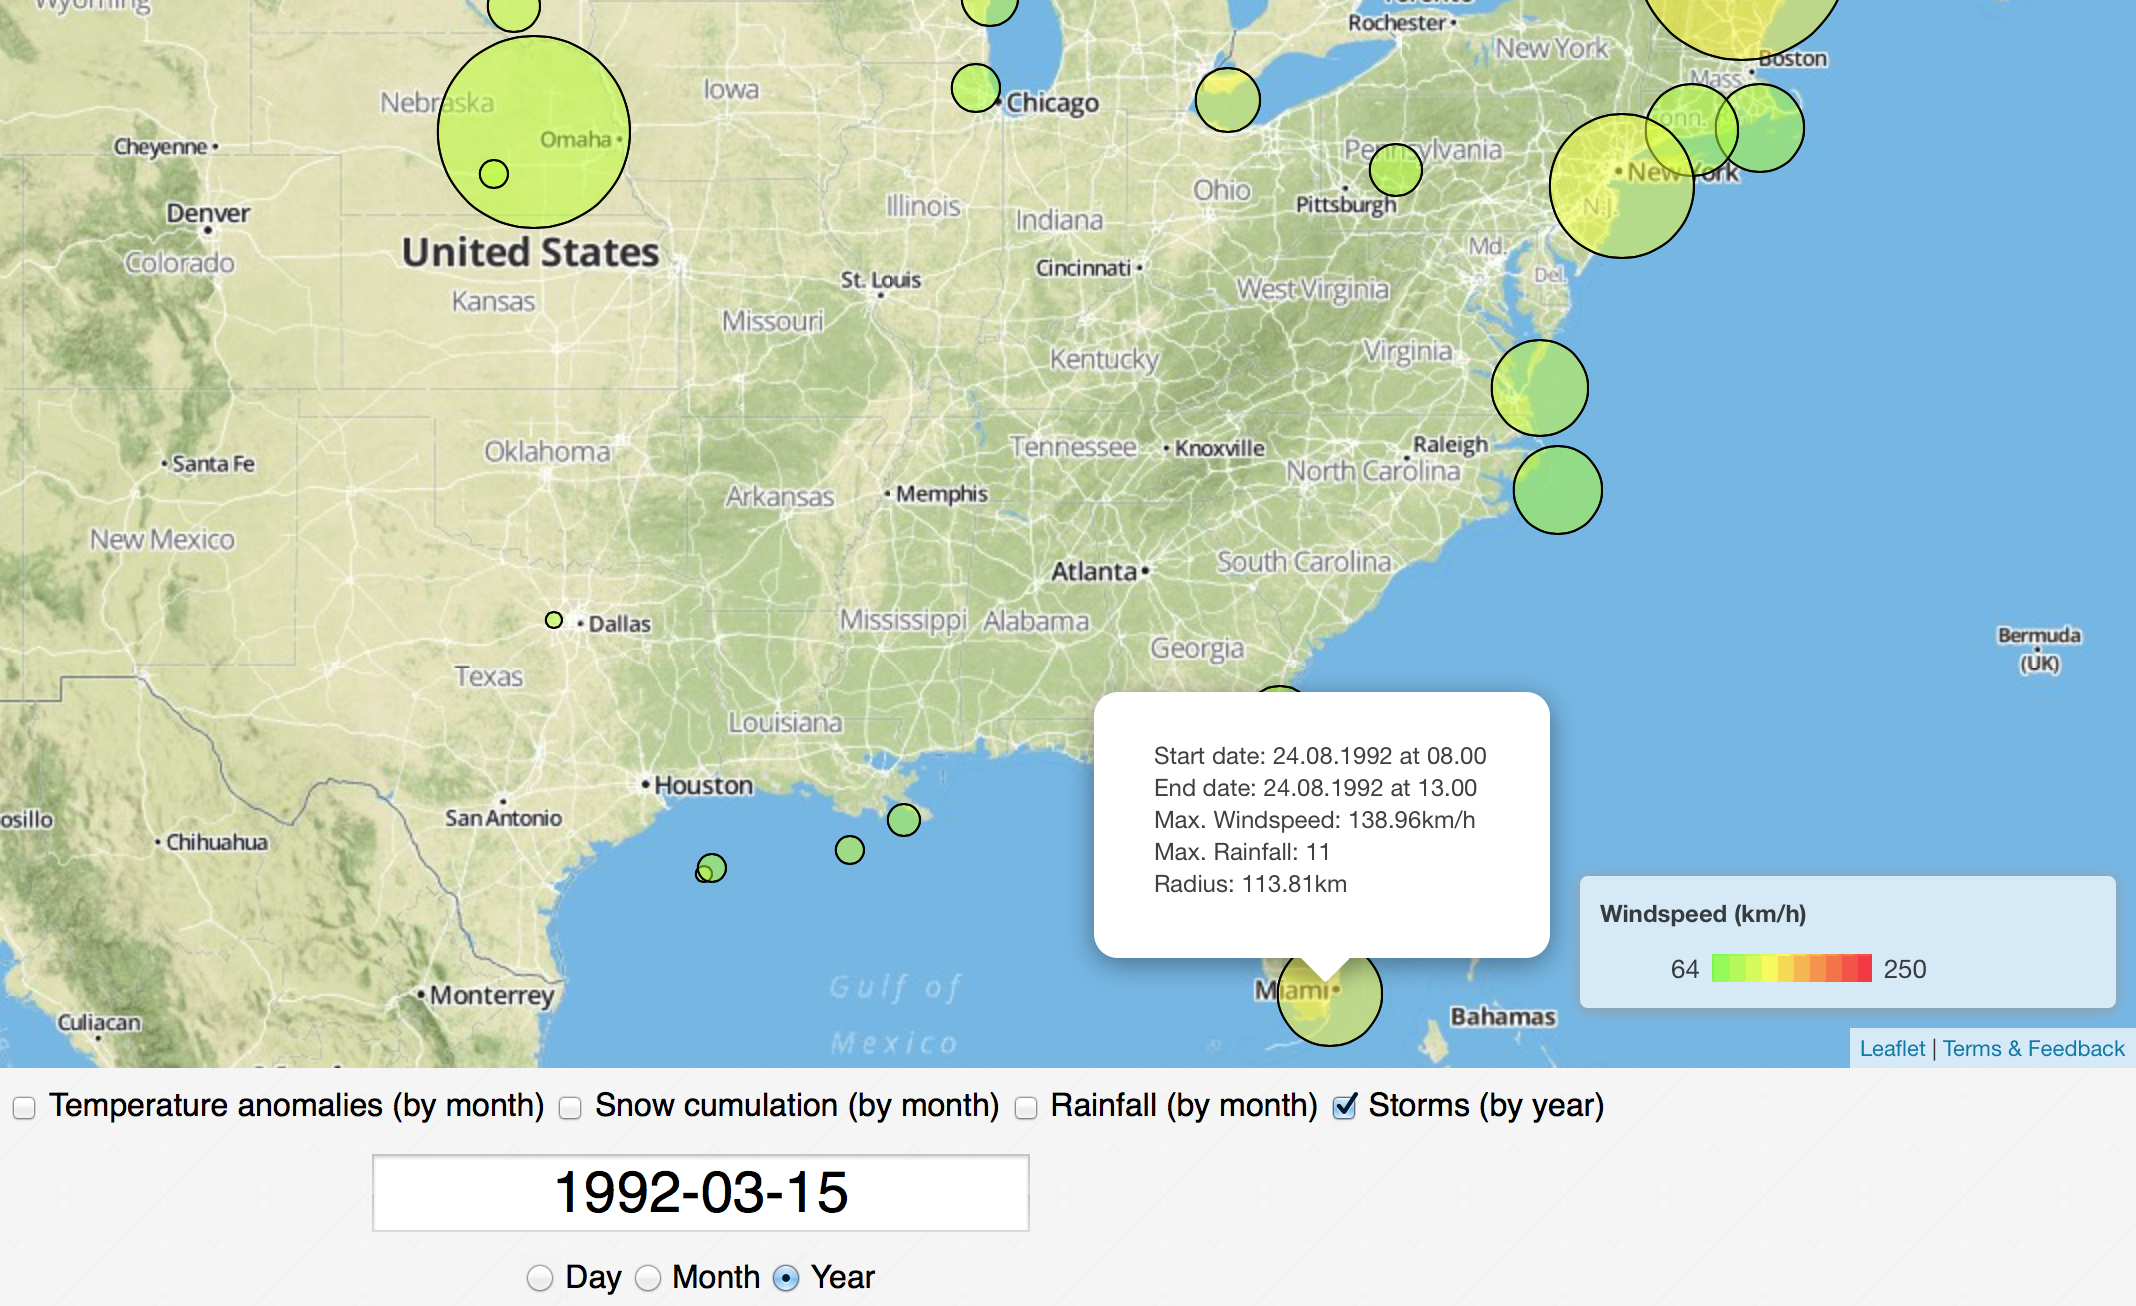
\includegraphics[width=17cm]{figures/wind1.png}
}
\caption{The wind storms on August 1992 zoomed in on Florida and New Orleans.}
\label{fig:rainfall1}
\end{figure}
\begin{figure}[ht]
\centering
\makebox[\textwidth][c]{
  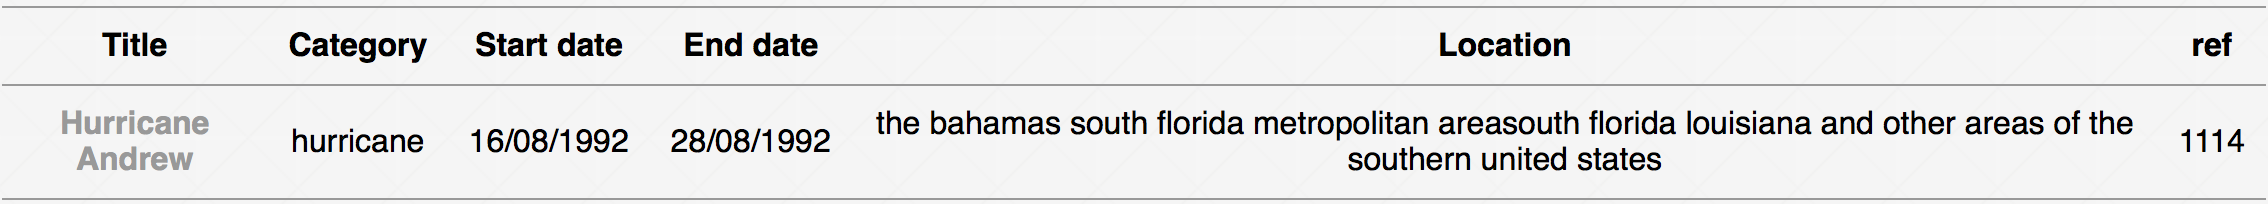
\includegraphics[width=17cm]{figures/wind2.png}
}
\caption{The wikipedia-report of hurricane Andrew}
\label{fig:rainfall2}
\end{figure}


%%%%%%%%%%%%%%%%%%%%%%%%%%%%%
\subsection{Inconsistent rain data}
There are extreme events that are also characterised by heavy rain. However, the retrieval of this information in the data set has caused us some important problems. In fact, the rain information was not always present in the same position as described in the official documentation for the dataset. Running our algorithms on the whole Swiss records worked perfectly, but once we executed it on the US, which is a much larger dataset, we encountered some exceptions. For example, instead of the amount of precipitations, we retrieved strings like \textit{?UML ?}, \textit{?O RM?}, etc. In the case of rainfall anomalies,  we even decided to switch dataset. For extreme events we continued to use the same dataset for compatibility with the wind and handled these exceptions as missing values.

%%%%%%%%%%%%%%%%%%%%%%%%%%%%%
\subsection{Missing information due to the impact of the event}
Some extreme events had such a big impact that we noticed that the stations recording data had been destroyed by the event. This has been the case for hurricane Katrina in 2005 for example, as the dataset presented an empty gap of almost  one month, on every station in the area of Katerina. For this reason there are extreme events that could not be recorded by the stations and cannot be found on the map. However we cannot deduce that if a lot of records are missing it is due to an extreme event. It could also be the station that has been inactivated or moved.

%%%%%%%%%%%%%%%%%%%%%%%%%%%%%
\subsection{Extreme events with low impact}
There are extreme events that can cause none or irrelevant impacts, like event in the middle of the desert, or only in the ocean. There is also events that match the characteristics of an extreme event but are actually pretty low and spreaded. For this reason there can be extreme events on the map without a match with Wikipedia articles.

%%%%%%%%%%%%%%%%%%%%%%%%%%%%%
\subsection{Extreme events and Wikipedia}
\begin{multicols}{2}
\begin{itemize}
\item Hurricane Eloise 1975 September
\item Hurricane Belle 1976 August
\item Hurricane Norman 1978 August
\item Hurricane David 1979 Aug-Sept
\item Hurricane Frederic 1979 Aug-Sept
\item Hurricane Alicia 1983 August
\item Hurricane Diana 1984 September
\item Hurricane Gloria 1985 September
\item Hurricane Juan	1985 October
\item Hurricane Charley 1986 August
\item Tropical Storm Beryl 1988 August
\item Hurricane Florence 1988 September	
\item Hurricane Chantal 1989 August
\item Hurricane Hugo 1989 September
\item Hurricane Bob 1991 August
\item Hurricane Andrew 1992 August
\item Hurricane Emily 1993 Aug-Sept
\item Hurricane Erin 1995 August
\item Hurricane Bertha 1996 July
\item Hurricane Fran 1996 Aug-Sept
\item Hurricane Bonnie 1998 August
\item Hurricane Georges 1998 September
\item Hurricane Bret 1999 August
\item Hurricane Floyd 1999 September
\item Hurricane Gabrielle 2001 September
\item Hurricane Isabel 2003 September
\item Tornado Nebraska 2004 May
\item Hurricane Charley 2004 August
\item Hurricane Ivan 2004 September
\item Hurricane Cindy 2005 July
\item Hurricane Rita 2005 September
\item Hurricane Ophelia 2005 September
\item Hurricane Wilma 2005 October
\item Tropical Storm Alberto 2006 June
\item Hurricane Ernesto 2006 August
\item Hurricane Humberto 2007 September
\item Great Coastal Gale of 2007 December
\item Hurricane Ike 2008 September
\item Hurricane Gustav 2008 September
\item Derecho Southern Midwest derecho 2009 May
\item Hurricane Irene 2011 August
\item Tropical Storm Lee 2011 September
\item Hurricane Isaac 2012 August
\item Hurricane sandy 2012 October
\item Tornado Outbreak 2013 November
\end{itemize}
\end{multicols}

%%%%%%%%%%%%%%%%%%%%%%%%%%%%%
\subsection{MapReduce jobs}
The goal of these MapReduce jobs is to find extreme events based principally on wind information. The final output will be composed of:
\begin{enumerate}
\item the start date of the event
\item the end date of the event
\item the coordinate of the center of the event
\item the radius of the event
\item the maximum wind speed recorded during the event
\item the maximum rain quantity that fall during the event
\end{enumerate}

\textbf{Mapper 1:} extract the following information from the input:
\begin{enumerate}
\item id of the station
\item date
\item geolocation of the station
\item wind speed
\item rain precipitation
\end{enumerate}
This information is sent to the reducer with one reducer per year/months (so two years give 24 reducer).

\textbf{Reducer 1:} analyse the wind speed. Output only if the wind is above a certain threshold, which signify that it is an extreme wind speed and therefore an extreme event.

We now have a huge list of extreme events. We need to know how long these events happened, how many days.

\textbf{Mapper 2:} send all data on one single mapper. We need all data on a single mapper because there is no way to know when an event is going to start or finish, therefore we cannot separate the data.

\textbf{Reducer 2:} sort all the date and then look for continuity. If there is a discontinuity of days between two inputs, we send all the previous events on the same key, which means we had one event. We then start the new event and look on how many days it happened.

We now have data that are classified by date. But maybe there are multiple events during this time. We have to make clusters of stations depending of their distance between each other

\textbf{Mapper 3:} send the data with a unique idea per event as key.

\textbf{Reducer 3:} for each continuous date we have a list of event. Some are part of the same event and happened close to each other, some not. We run a clustering algorithm in order to make different clusters for each event.

We now have a set of clusters, each cluster representing an event. We want to extract information from these clusters.

\textbf{Mapper 4:} distributes values between reducers.

\textbf{Reducer 4:} last process in order to find the elements listed in the output list above. This output will then be given to a post-processing script in order to create GeoJSON for the visualisation of the data.
